\begin{figure}
    \begin{center}
    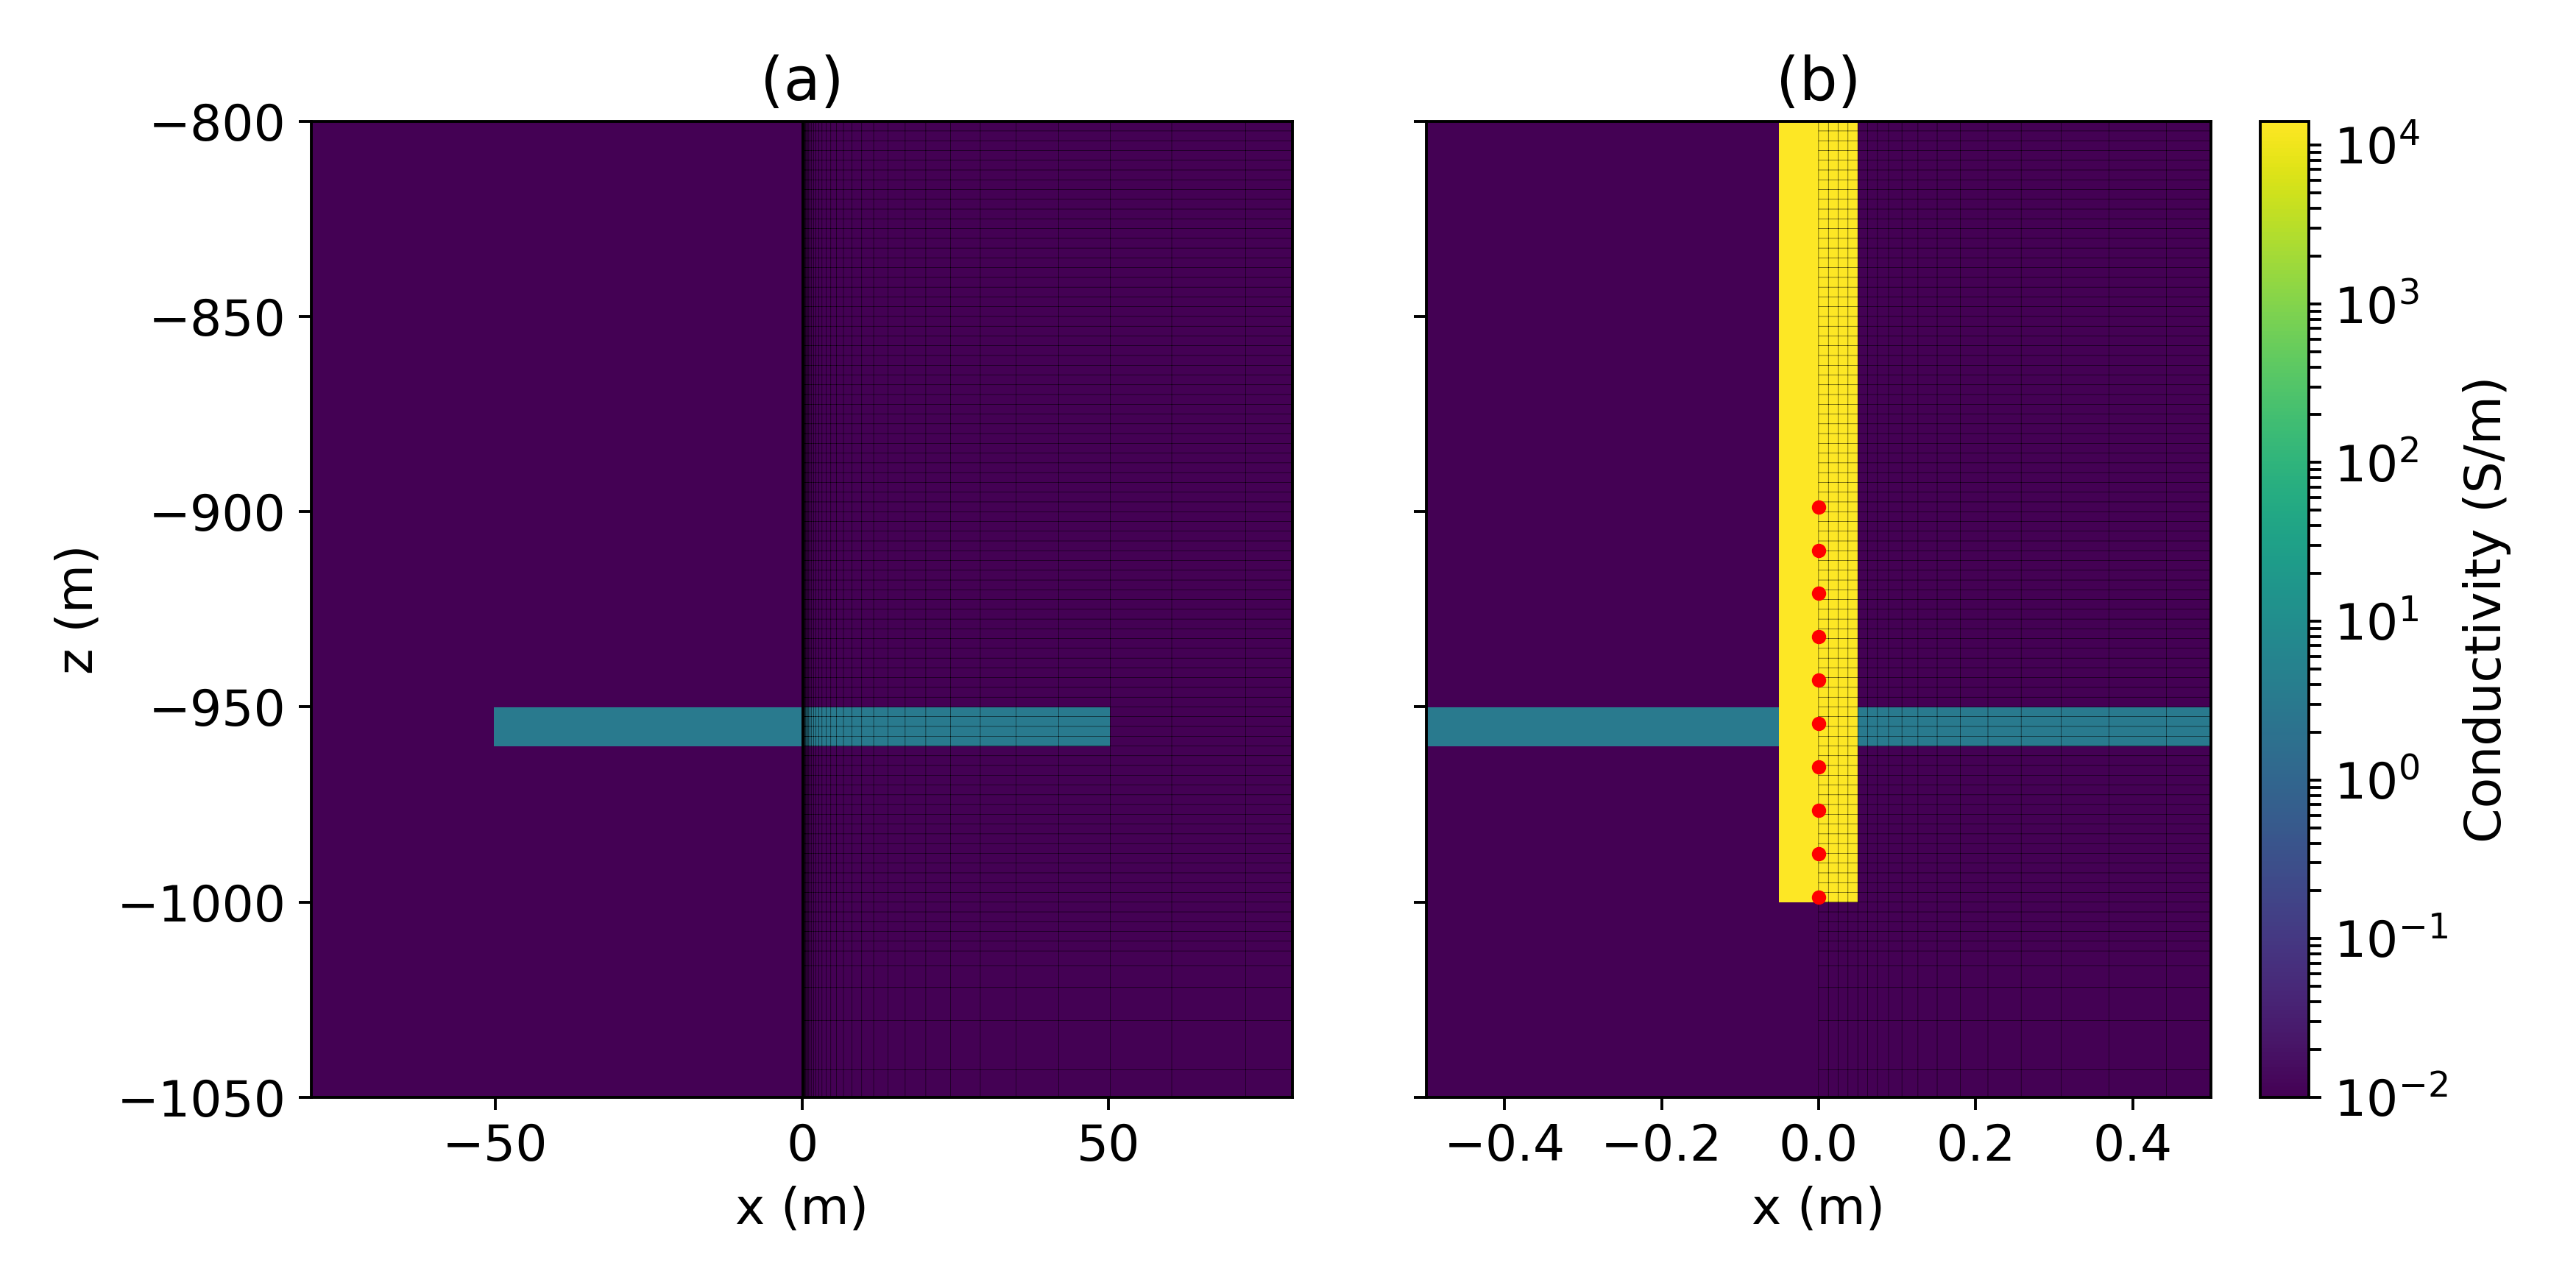
\includegraphics[width=\textwidth]{figures/inversion/DC_cyl_setup.png}
    \end{center}
\caption{
    Model of an electrically conductive propped fracture zone (3 S/m) in a halfspace (100 $\Omega$ m) with a steel-cased well.
    The well is modelled as a solid cylinder with a conductivity of $1.4 \times 10^4$ S/m. The mesh has 4 cells across the
    radius of the casing. The fractured region extends vertically from 950 to 960 m depth and has a radius of 50m.
    Panel (a) has a radial extent of 80 m to show the fractured zone and panel (b) has a radius of 0.4m to show the casing.
    The a-electrode locations are shown in panel (b).
}
\label{fig:DC_cyl_setup}
\end{figure}
